\documentclass[11pt]{article}

% ----- Packages -----
\usepackage[a4paper,margin=1.1in]{geometry}
\usepackage[T1]{fontenc}
\usepackage[utf8]{inputenc}
\usepackage{lmodern}
\usepackage{microtype}
\usepackage{booktabs}
\usepackage{tabularx}
\usepackage{array}
\usepackage{enumitem}
\usepackage{amsmath}
\usepackage{amssymb}
\usepackage{xcolor}
\usepackage{titlesec}
\usepackage{tikz}
\usetikzlibrary{arrows.meta,positioning,decorations.pathreplacing,fit,calc}
\usepackage[hidelinks]{hyperref}

% ----- Style -----
\definecolor{ergoorange}{HTML}{FF5E18}
\definecolor{rulegray}{HTML}{888888}

\titleformat{\section}{\Large\bfseries}{\thesection}{0.8em}{}
\titleformat{\subsection}{\large\bfseries}{\thesubsection}{0.8em}{}

\setlist{itemsep=2pt,topsep=4pt}

\newcommand{\name}[1]{\texttt{\textasciitilde#1}}
\newcommand{\code}[1]{\texttt{#1}}

\hypersetup{
  pdftitle={ErgoNames: A Decentralized Naming Protocol on Ergo},
  pdfauthor={ErgoNames},
  pdfsubject={Whitepaper},
}

\begin{document}

% ================= Title =================
\begin{titlepage}
  \centering
  \vspace*{2.5cm}
  {\color{ergoorange}\rule{\textwidth}{2pt}}\\[1.2cm]
  {\Huge\bfseries ErgoNames}\\[0.6cm]
  {\LARGE A Decentralized Naming Protocol on Ergo}\\[1.2cm]
  {\color{ergoorange}\rule{\textwidth}{2pt}}\\[2cm]
  {\large Version 1.0 --- Draft}\\[0.4cm]
  {\large June 2026}\\
  \vfill
  {\large \href{https://ergonames.io}{ergonames.io}}\\[0.3cm]
  {\small Contracts: \href{https://github.com/ergonames/ergonames-contracts}{github.com/ergonames/ergonames-contracts}}
\end{titlepage}

% ================= Abstract =================
\begin{abstract}
\noindent
ErgoNames is a decentralized naming protocol built natively on the Ergo
blockchain. It maps human-readable names (e.g.\ \name{adoo}) to Ergo
addresses and arbitrary on-chain identities, with each name issued as a
non-fungible token (NFT) under a \emph{lifetime-ownership} model: a name is
bought once, owned forever, and freely transferable --- there are no renewal
fees and no expiry.

The protocol is implemented entirely in ErgoScript on Ergo's extended-UTXO
(eUTXO) model. A single on-chain registry box, carrying an authenticated AVL
tree, guarantees global name uniqueness without any trusted intermediary.
Registration uses a commit--reveal scheme to prevent front-running, prices
names in USD via a decentralized ERG/USD oracle, and embeds the name's
artwork directly on-chain as an SVG --- no external hosting, IPFS, or mutable
metadata. Every name additionally anchors its own subname registry, enabling
hierarchical names (\code{sub\textasciitilde name}) controlled by the parent
name's holder.

This paper describes the protocol's design goals, contract architecture,
registration flow, pricing mechanism, refund and fund-safety guarantees, and
upgrade path.
\end{abstract}

\vspace{0.5cm}
\tableofcontents
\newpage

% ================= 1 =================
\section{Introduction}

\subsection{Motivation}

Blockchain addresses are long, unmemorable, and error-prone. A naming layer
--- analogous to DNS for the internet --- is foundational infrastructure for
payments, identity, and applications. Ethereum's ENS demonstrated demand for
such a layer, but its design carries assumptions that do not fit every chain
or every user:

\begin{itemize}
  \item \textbf{Rental, not ownership.} ENS names expire and must be renewed;
        a lapsed renewal can mean losing an identity (and everything pointed
        at it) to a squatter.
  \item \textbf{Account-model implementation.} ENS relies on mutable contract
        storage and a resolver-contract hierarchy that has no direct analogue
        in UTXO systems.
\end{itemize}

ErgoNames takes the opposite stance on the first point and solves the second
natively: names are \emph{owned for life}, and the entire registry lives in
Ergo's eUTXO model using on-chain authenticated data structures rather than
contract storage.

\subsection{Design goals}

\begin{enumerate}
  \item \textbf{Lifetime ownership.} One purchase, permanent ownership. A name
        is an NFT in the user's wallet; holding the token \emph{is} owning the
        name.
  \item \textbf{Global uniqueness, trustlessly enforced.} No two identical
        names can ever be minted. Uniqueness is enforced by consensus, not by
        an off-chain operator.
  \item \textbf{Front-running resistance.} Observing a pending registration in
        the mempool must not allow an attacker to steal the name.
  \item \textbf{Fund safety at every step.} Registration is a
        multi-transaction process; at every intermediate stage the user's
        funds must be recoverable by the user alone, without operator
        cooperation.
  \item \textbf{Fully on-chain artifacts.} Name metadata and artwork are
        stored on-chain. Nothing about a name depends on a server staying up.
  \item \textbf{Stable, predictable pricing.} Names are priced in USD by
        length, converted to ERG at mint time via a decentralized oracle.
  \item \textbf{Upgradability without custody.} Protocol parameters and
        contract logic can evolve via a multisig escape hatch --- but the
        operator can never confiscate, modify, or expire an already-minted
        name, because minted names are ordinary tokens in user wallets.
\end{enumerate}

% ================= 2 =================
\section{Background: Ergo and the eUTXO Model}

Ergo is a proof-of-work blockchain whose transaction model extends Bitcoin's
UTXO design. Key primitives used by ErgoNames:

\begin{itemize}
  \item \textbf{Boxes.} The unit of state. A box holds ERG, tokens, and up to
        ten typed registers (R4--R9), and is guarded by an ErgoScript contract
        that must evaluate to true for the box to be spent.
  \item \textbf{Tokens and singletons.} Ergo supports native tokens minted
        in-transaction. A token with supply 1 (a \emph{singleton}) uniquely
        identifies a logical entity across box generations: when the registry
        box is spent and recreated, the singleton proves the new box is the
        same registry.
  \item \textbf{Authenticated AVL trees.} Ergo natively supports
        cryptographically authenticated dictionaries (AVL+ trees). A box
        register stores only the tree's digest ($\approx$33 bytes); off-chain
        actors supply insertion/lookup proofs that the contract verifies
        on-chain. This gives ErgoNames an unbounded key--value registry with
        constant on-chain footprint.
  \item \textbf{Data inputs.} Transactions can \emph{reference} boxes without
        spending them. ErgoNames reads the ERG/USD oracle this way, so price
        feeds are consumed without contention.
  \item \textbf{Sigma propositions.} Spending conditions are sigma-protocol
        statements, enabling native threshold signatures
        (\code{atLeast(k, \ldots)}) used for the protocol's multisig escape
        hatches.
\end{itemize}

These primitives are the reason ErgoNames needs no resolver-contract
hierarchy: the registry is one box, the proof system enforces uniqueness, and
ownership is plain token custody.

% ================= 3 =================
\section{Protocol Overview}

\subsection{Names}

An ErgoName is a string of one or more characters drawn from
\code{[a-z A-Z 0-9 \_]} (the X/Twitter handle alphabet), rendered with a
leading tilde by convention: \name{adoo}. Validity is enforced
\textbf{on-chain} --- the registry contract checks every byte of the name
against the allowed ASCII ranges before permitting a mint.

A registered name is an
EIP-4\footnote{\url{https://github.com/ergoplatform/eips/blob/master/eip-0004.md}}
picture NFT belonging to the official ErgoNames collection (EIP-34). Its
artwork --- a rendered card showing the name --- is generated
deterministically and embedded in the token's registers as a base64
\code{data:image/svg+xml} URI together with its SHA-256 hash. The NFT is
self-contained: wallets and marketplaces can display it with zero external
dependencies, forever.

\subsection{Resolution and reverse resolution}

\begin{itemize}
  \item \textbf{Forward resolution} (\name{name} $\rightarrow$ address): the
        current holder of the name token \emph{is} the resolved address.
        Resolution is therefore live and automatic --- transferring the NFT
        re-points the name, with no separate ``set resolver'' step and no
        stale records.
  \item \textbf{Reverse resolution} (address $\rightarrow$ names): an indexer
        enumerates names held by an address, with a user-designated primary
        name.
\end{itemize}

Because resolution is defined by token custody, it inherits all of Ergo's
wallet semantics: names can sit in cold storage, multisig vaults, or smart
contracts, and ``who owns this name'' is always answerable from the UTXO set
alone.

\subsection{On-chain components}

The protocol consists of a small set of long-lived singleton boxes and
per-registration ephemeral boxes (Table~\ref{tab:components}).

\begin{table}[ht]
  \centering
  \small
  \begin{tabularx}{\textwidth}{@{}l l X@{}}
    \toprule
    \textbf{Component} & \textbf{Kind} & \textbf{Role} \\
    \midrule
    Registry & singleton box & Authoritative name set (AVL tree digest),
      price map, commit-age window; validates every mint \\
    \addlinespace
    Collection & singleton box & Holds the EIP-34 collection token supply;
      exactly one collection token is consumed per minted name, tying every
      name verifiably to the official collection \\
    \addlinespace
    Config & singleton box & On-chain updatable parameter store (AVL tree),
      reserved for alternative payment options \\
    \addlinespace
    Subname registry & one singleton per name & Anchors the subname tree for
      each registered name (\S\ref{sec:subnames}) \\
    \addlinespace
    Fee split & accumulator contract & Receives mint fees; enforces per-mille
      distribution to configured recipients \\
    \addlinespace
    Commit / Reveal-proxy / Reveal & ephemeral boxes & Per-registration boxes
      implementing the commit--reveal flow (\S\ref{sec:mintflow}) \\
    \bottomrule
  \end{tabularx}
  \caption{On-chain components of the ErgoNames protocol.}
  \label{tab:components}
\end{table}

The registry's AVL tree maps $\mathrm{blake2b256}(\mathit{name}) \rightarrow
\mathit{name\ token\ ID}$. Inserting a key that already exists is
cryptographically impossible to prove, so \textbf{uniqueness is a consequence
of the proof system itself}, not of any operator behaving honestly.

% ================= 4 =================
\section{Registration: The Commit--Reveal Mint Flow}
\label{sec:mintflow}

Na\"ive on-chain registration is front-runnable: an attacker watching the
mempool sees the desired name and submits a competing registration with a
higher fee. ErgoNames eliminates this with a two-phase commit--reveal scheme
split across four transactions. The first two are built and signed
\textbf{by the user in their own wallet}; the last two are executed by a
permissionless off-chain transaction operator (``bot'').

\begin{figure}[ht]
\centering
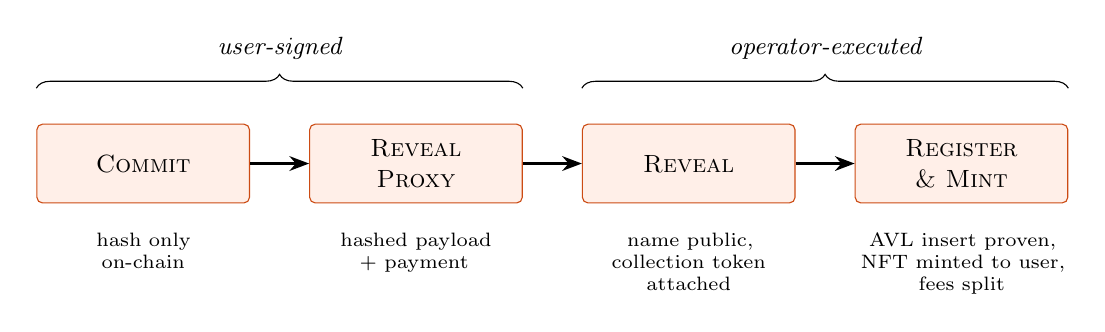
\begin{tikzpicture}[
  txbox/.style={draw=ergoorange!80!black, fill=ergoorange!10, rounded corners=2pt,
    minimum width=2.7cm, minimum height=1.0cm, align=center, font=\small\scshape},
  note/.style={font=\scriptsize, align=center, text width=2.7cm},
  arr/.style={-{Stealth[length=2.5mm]}, thick}
]
  \node[txbox] (commit) {Commit};
  \node[txbox, right=0.75cm of commit] (proxy) {Reveal\\Proxy};
  \node[txbox, right=0.75cm of proxy] (reveal) {Reveal};
  \node[txbox, right=0.75cm of reveal] (register) {Register\\\& Mint};

  \draw[arr] (commit) -- (proxy);
  \draw[arr] (proxy) -- (reveal);
  \draw[arr] (reveal) -- (register);

  \node[note, below=0.25cm of commit] {hash only\\on-chain};
  \node[note, below=0.25cm of proxy] {hashed payload\\+ payment};
  \node[note, below=0.25cm of reveal] {name public,\\collection token\\attached};
  \node[note, below=0.25cm of register] {AVL insert proven,\\NFT minted to user,\\fees split};

  \draw[decorate, decoration={brace, amplitude=5pt}]
    ([yshift=0.45cm]commit.north west) -- ([yshift=0.45cm]proxy.north east)
    node[midway, above=7pt, font=\small\itshape] {user-signed};
  \draw[decorate, decoration={brace, amplitude=5pt}]
    ([yshift=0.45cm]reveal.north west) -- ([yshift=0.45cm]register.north east)
    node[midway, above=7pt, font=\small\itshape] {operator-executed};
\end{tikzpicture}
\caption{The four-transaction registration flow. The user signs the first
two transactions in their own wallet; the off-chain operator executes the
last two against the registry.}
\label{fig:mintflow}
\end{figure}

\paragraph{1. Commit.}
The user creates a commit box containing their public key and the commitment
\[
  \mathrm{blake2b256}(\mathit{secret} \,\Vert\, \mathit{userPK} \,\Vert\,
  \mathit{nameBytes}).
\]
Nothing about the name is revealed. The registry enforces a commit
\textbf{age window} ($\mathit{minAge}$, $\mathit{maxAge}$): the commit must
mature for a minimum
number of blocks before it can be consumed (so an attacker cannot observe a
reveal and out-commit it retroactively), and expires after a maximum age.

\paragraph{2. Reveal proxy.}
The user funds a proxy box carrying the full registration payment plus
operator/miner fees, and a binding hash of the exact reveal box to be
created. The plaintext name still does not appear on-chain; it travels to the
operator off-chain.

\paragraph{3. Reveal.}
The operator spends the proxy together with the collection box, producing a
reveal box that now carries the name, the user's secret, the commit box
reference, the EIP-4 artwork registers, and \textbf{one collection token}
borrowed from the collection box. The reveal box's contents are constrained
byte-exactly by the hash committed in step 2 --- the operator cannot alter
the name, the recipient, or the fees.

\paragraph{4. Register \& mint.}
The final transaction spends the reveal, registry, and commit boxes together.
The registry contract verifies, in consensus:

\begin{itemize}
  \item the commit hash matches
        $\mathrm{blake2b256}(\mathit{secret} \,\Vert\, \mathit{userPK}
        \,\Vert\, \mathit{nameBytes})$ --- proving this user committed to this
        name before revealing it;
  \item the commit box age lies within the registry's age window;
  \item the name is valid ASCII (\S3.1);
  \item the supplied \textbf{AVL insertion proof} transitions the registry
        digest by inserting exactly
        $\mathrm{blake2b256}(\mathit{name}) \rightarrow \mathit{tokenId}$,
        which fails if the name already exists;
  \item the payment covers the oracle-derived price
        (\S\ref{sec:pricing}) and is routed to the fee-split contract;
  \item the new name NFT (carrying the on-chain SVG and collection linkage)
        is delivered to the committed user's public key;
  \item a fresh \textbf{subname registry} box is created for the name
        (\S\ref{sec:subnames});
  \item the recreated registry box preserves the singleton, the updated tree,
        and all parameters.
\end{itemize}

\begin{figure}[ht]
\centering
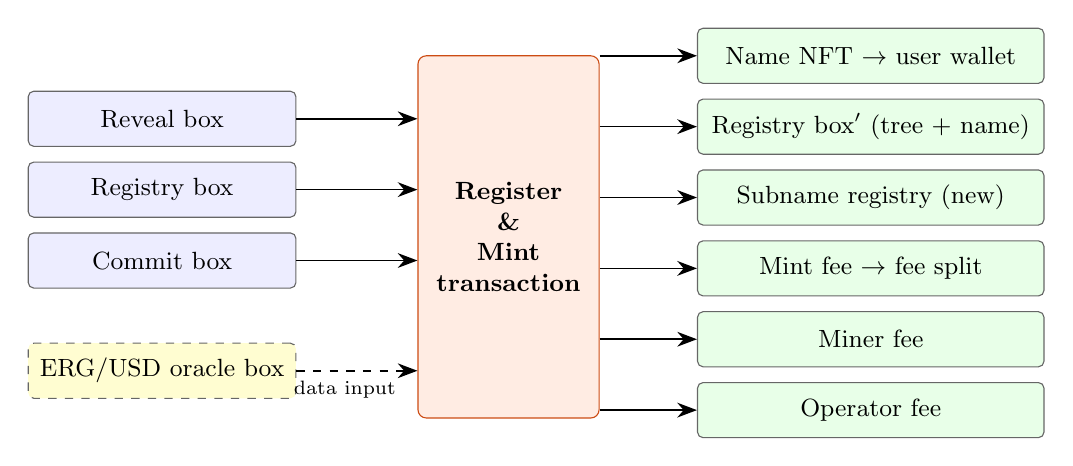
\begin{tikzpicture}[
  inbox/.style={draw=black!60, fill=blue!7, rounded corners=2pt,
    minimum width=3.4cm, minimum height=0.7cm, align=center, font=\small},
  outbox/.style={draw=black!60, fill=green!9, rounded corners=2pt,
    minimum width=4.4cm, minimum height=0.7cm, align=center, font=\small},
  databox/.style={draw=black!60, dashed, fill=yellow!18, rounded corners=2pt,
    minimum width=3.4cm, minimum height=0.7cm, align=center, font=\small},
  txnode/.style={draw=ergoorange!80!black, fill=ergoorange!12, rounded corners=3pt,
    minimum width=2.3cm, minimum height=4.6cm, align=center, font=\small\bfseries},
  arr/.style={-{Stealth[length=2.5mm]}, semithick},
  darr/.style={-{Stealth[length=2.5mm]}, semithick, dashed}
]
  \node[txnode] (tx) at (0,0) {Register\\\&\\Mint\\transaction};

  \node[inbox]   (in1) at (-4.4,  1.5) {Reveal box};
  \node[inbox]   (in2) at (-4.4,  0.6) {Registry box};
  \node[inbox]   (in3) at (-4.4, -0.3) {Commit box};
  \node[databox] (din) at (-4.4, -1.7) {ERG/USD oracle box};

  \node[outbox] (o1) at (4.6,  2.3) {Name NFT $\rightarrow$ user wallet};
  \node[outbox] (o2) at (4.6,  1.4) {Registry box$'$ (tree + name)};
  \node[outbox] (o3) at (4.6,  0.5) {Subname registry (new)};
  \node[outbox] (o4) at (4.6, -0.4) {Mint fee $\rightarrow$ fee split};
  \node[outbox] (o5) at (4.6, -1.3) {Miner fee};
  \node[outbox] (o6) at (4.6, -2.2) {Operator fee};

  \draw[arr] (in1.east) -- (tx.west |- in1.east);
  \draw[arr] (in2.east) -- (tx.west |- in2.east);
  \draw[arr] (in3.east) -- (tx.west |- in3.east);
  \draw[darr] (din.east) -- node[below, font=\scriptsize, pos=0.4] {data input}
    (tx.west |- din.east);

  \draw[arr] (tx.east |- o1.west) -- (o1.west);
  \draw[arr] (tx.east |- o2.west) -- (o2.west);
  \draw[arr] (tx.east |- o3.west) -- (o3.west);
  \draw[arr] (tx.east |- o4.west) -- (o4.west);
  \draw[arr] (tx.east |- o5.west) -- (o5.west);
  \draw[arr] (tx.east |- o6.west) -- (o6.west);
\end{tikzpicture}
\caption{Anatomy of the register \& mint transaction. The oracle box is
referenced read-only (data input), so price reads never contend with other
transactions. The registry box is recreated with the singleton, updated AVL
tree, and unchanged parameters.}
\label{fig:txanatomy}
\end{figure}

The token is minted with two units: one to the user's wallet (the ownership
token) and one bound into the name's subname registry box, permanently
linking the name to its subname tree.

\paragraph{Front-running analysis.}
Before step 4, the name appears on-chain only as hashes. An attacker who
learns the name at reveal time cannot register it, because they cannot
produce a commit box older than $\mathit{minAge}$ blocks that hashes to a
commitment over \emph{their} key --- the age window makes retroactive
commitment impossible. Two honest users racing for the same name are
serialized by the registry singleton: exactly one insertion proof can
succeed, and the loser is refunded (\S\ref{sec:refunds}).

% ================= 5 =================
\section{Pricing}
\label{sec:pricing}

Names are priced \textbf{in USD by character length}, with shorter names
costing more, and settled in ERG at the prevailing market rate:

\begin{itemize}
  \item The registry box carries a \textbf{price map}: a vector where index
        $n$ is the USD price for an $n$-character name (the last entry covers
        all longer names).
  \item At mint time, the transaction must reference the \textbf{SigUSD
        ERG/USD oracle pool box as a data input}. The registry computes
        $\mathit{fee} = \mathit{nanoErgPerUsd} \times \mathit{price}$ from the
        oracle's current datapoint and requires the payment output to cover
        it (within a bounded slippage window, since the oracle may update
        between quote and confirmation).
  \item The price map is an on-chain register, updatable by the protocol
        multisig via the escape hatch (\S\ref{sec:governance})
        \textbf{without redeploying the registry} --- pricing policy can
        evolve while the name set, singleton, and history remain untouched.
\end{itemize}

Because the oracle is a data input, price reads are contention-free, and
because the conversion happens inside the contract, the operator cannot
overcharge: a user who pays the on-chain-computed fee gets the name, period.
The architecture also reserves support (via the config box and oracle data
inputs) for payment in tokens other than ERG.

There are \textbf{no recurring fees}. The mint fee is the only payment a name
holder ever makes.

% ================= 6 =================
\section{Subnames}
\label{sec:subnames}

Every registered name owns a hierarchical namespace beneath it. The mint
transaction creates a dedicated \textbf{subname registry} box for the new
name --- a singleton carrying its own AVL tree and a unit of the parent
name's token, cryptographically binding the subname tree to the parent.

The holder of the parent name NFT can:

\begin{itemize}
  \item \textbf{mint subnames} (\code{pay}, \code{vault}, \ldots\ under
        \name{adoo}), each itself an NFT with its own child subname registry
        --- the hierarchy nests to arbitrary depth;
  \item \textbf{revoke a child subname} (parent burns child), preserving the
        parent's authority over its namespace;
\end{itemize}

and a subname holder can \textbf{self-burn} their subname. All three
operations are enforced by the subname registry contract with the same
AVL-proof machinery as the root registry: uniqueness within each namespace
level is consensus-enforced.

This supports organizational identity (\code{alice} under \name{mycompany}),
service endpoints, and delegated naming, while keeping the root registry's
economics intact.

\begin{figure}[ht]
\centering
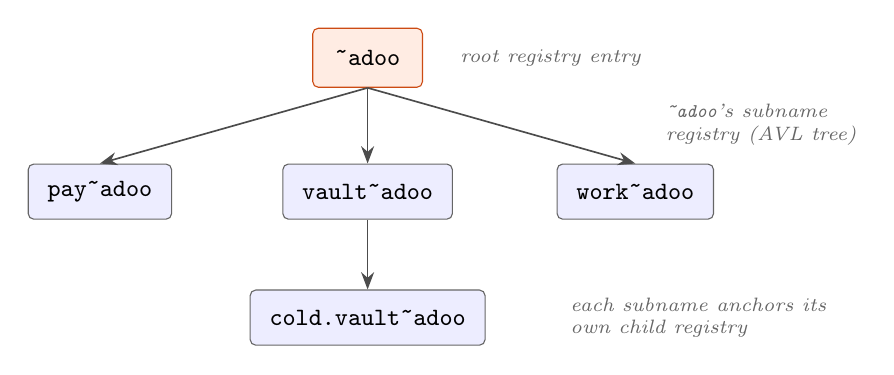
\begin{tikzpicture}[
  root/.style={draw=ergoorange!80!black, fill=ergoorange!12, rounded corners=2pt,
    minimum height=0.75cm, inner xsep=8pt, font=\small\ttfamily},
  nm/.style={draw=black!60, fill=blue!7, rounded corners=2pt,
    minimum height=0.7cm, inner xsep=7pt, font=\small\ttfamily},
  reg/.style={font=\scriptsize\itshape, text=black!60},
  arr/.style={-{Stealth[length=2.2mm]}, semithick, black!70}
]
  \node[root] (parent) at (0,0) {\textasciitilde adoo};
  \node[reg, right=0.35cm of parent] {root registry entry};

  \node[nm] (pay)   at (-3.4,-1.7) {pay\textasciitilde adoo};
  \node[nm] (vault) at (0,-1.7)    {vault\textasciitilde adoo};
  \node[nm] (work)  at (3.4,-1.7)  {work\textasciitilde adoo};

  \node[nm] (cold) at (0,-3.3) {cold.vault\textasciitilde adoo};

  \draw[arr] (parent.south) -- (pay.north);
  \draw[arr] (parent.south) -- (vault.north);
  \draw[arr] (parent.south) -- (work.north);
  \draw[arr] (vault.south) -- (cold.north);

  \node[reg, align=left] at (5.0,-0.85)
    {\name{adoo}'s subname\\registry (AVL tree)};
  \node[reg, align=left] at (4.2,-3.3)
    {each subname anchors its\\own child registry};
\end{tikzpicture}
\caption{Hierarchical subnames. Each registered name carries a singleton
subname registry; every subname is itself an NFT that anchors a child
registry, nesting to arbitrary depth. The parent's holder can mint and revoke
children.}
\label{fig:subnames}
\end{figure}

% ================= 7 =================
\section{Fund Safety and Refunds}
\label{sec:refunds}

Registration spans multiple transactions, so the protocol is explicit about
every intermediate state. \textbf{Each ephemeral box is refundable by the
user's signature alone} --- the operator can never strand or seize in-flight
funds:

\begin{itemize}
  \item \textbf{Commit refund.} After the commit's maximum age passes, the
        user can reclaim the commit box to their own key.
  \item \textbf{Reveal-proxy refund.} The user can unwind an unprocessed
        proxy box, recovering the full payment.
  \item \textbf{Reveal refund.} If a reveal can no longer complete (e.g.\ the
        name was registered first by someone else), the user reclaims the
        reveal box's value; the transaction simultaneously \textbf{returns
        the borrowed collection token} to the collection box, preserving the
        collection-supply invariant.
\end{itemize}

\begin{figure}[ht]
\centering
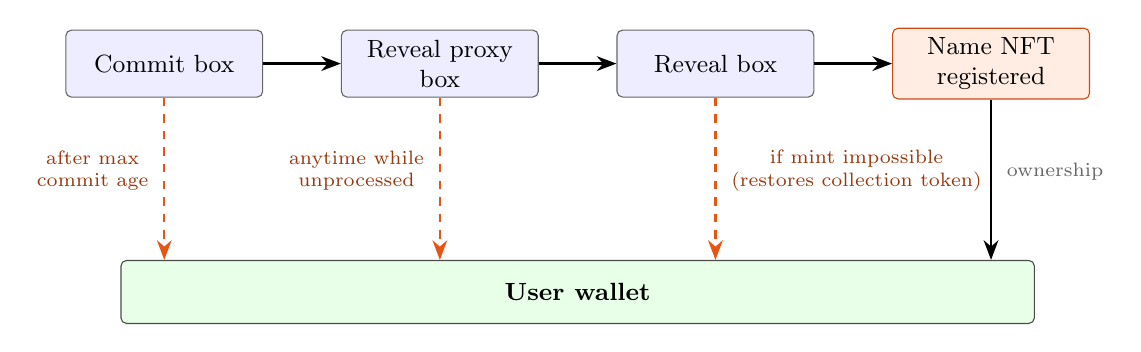
\begin{tikzpicture}[
  stage/.style={draw=black!60, fill=blue!7, rounded corners=2pt,
    minimum width=2.5cm, minimum height=0.85cm, align=center, font=\small},
  final/.style={draw=ergoorange!80!black, fill=ergoorange!12, rounded corners=2pt,
    minimum width=2.5cm, minimum height=0.85cm, align=center, font=\small},
  wallet/.style={draw=black!70, fill=green!9, rounded corners=2pt,
    minimum width=11.6cm, minimum height=0.8cm, align=center, font=\small\bfseries},
  arr/.style={-{Stealth[length=2.5mm]}, thick},
  refund/.style={-{Stealth[length=2.5mm]}, thick, dashed, ergoorange!90!black},
  rlbl/.style={font=\scriptsize, align=center, ergoorange!60!black}
]
  \node[stage] (commit) at (0,0)    {Commit box};
  \node[stage] (proxy)  at (3.5,0)  {Reveal proxy\\box};
  \node[stage] (reveal) at (7.0,0)  {Reveal box};
  \node[final] (done)   at (10.5,0) {Name NFT\\registered};

  \draw[arr] (commit) -- (proxy);
  \draw[arr] (proxy) -- (reveal);
  \draw[arr] (reveal) -- (done);

  \node[wallet] (wallet) at (5.25,-2.9) {User wallet};

  \draw[refund] (commit.south) -- node[rlbl, left=2pt, pos=0.45]
    {after max\\commit age} (commit.south |- wallet.north);
  \draw[refund] (proxy.south) -- node[rlbl, left=2pt, pos=0.45]
    {anytime while\\unprocessed} (proxy.south |- wallet.north);
  \draw[refund] (reveal.south) -- node[rlbl, right=2pt, pos=0.45]
    {if mint impossible\\(restores collection token)}
    (reveal.south |- wallet.north);
  \draw[arr] (done.south) -- node[rlbl, right=2pt, pos=0.45, black!60]
    {ownership} (done.south |- wallet.north);
\end{tikzpicture}
\caption{Refund paths (dashed). Every intermediate box is recoverable by the
user's signature alone; the operator can neither strand nor seize in-flight
funds. The successful path ends with the name NFT in the same wallet.}
\label{fig:refunds}
\end{figure}

Conversely, refunds \emph{require} the user's signature: the operator cannot
redirect a refund to itself. Races for the same name therefore resolve
cleanly --- one party gets the name, the other gets their money back, and no
third outcome exists.

The collection token supply decreases by exactly one per successful mint and
is restored by every refund, making the total number of names ever minted
auditable directly from the collection box.

% ================= 8 =================
\section{Governance and Upgradability}
\label{sec:governance}

ErgoNames separates what must be immutable from what must be able to evolve:

\begin{itemize}
  \item \textbf{Minted names are beyond protocol control.} A name NFT is an
        ordinary token in a user wallet. No multisig, upgrade, or migration
        can confiscate, alter, or expire it. Lifetime ownership is
        structural, not a policy promise.
  \item \textbf{Protocol boxes carry a multisig escape hatch.} The registry,
        subname registries, collection, config, and fee-split boxes can each
        be spent by a threshold signature of the protocol keys --- but
        \textbf{only in transaction shapes that are not mints}. The contracts
        structurally distinguish mint-shaped transactions (which must satisfy
        the full validation logic regardless of any signature) from
        migration-shaped ones (which fall through to the multisig). The
        multisig therefore cannot be used to mint names that bypass
        validation; it can only re-point a box to revised contract logic.
  \item \textbf{Upgrades preserve state.} Because the registry's identity is
        its singleton token --- not its script hash --- a migration moves the
        AVL tree, price map, and history into a box with new logic while
        every existing name, proof, and reference remains valid. Parameter
        changes (pricing, fee recipients, age window) are register-level
        updates requiring no logic change at all.
  \item \textbf{Fee distribution is contract-enforced.} Mint fees accumulate
        in the fee-split contract, spendable only by a transaction paying
        every configured recipient at least its per-mille share. Revenue
        policy (e.g.\ a future dev/treasury/DAO split) is a config change,
        not a custody change.
\end{itemize}

This yields a credible path from the current founder-operated multisig toward
progressively decentralized key holding, without ever touching user-owned
names.

% ================= 9 =================
\section{Off-Chain Architecture}

The chain enforces all rules; off-chain components only provide convenience
and liveness. The reference stack:

\begin{itemize}
  \item \textbf{Transaction operator (bot).} A stateless-by-design daemon
        that watches pending registrations and executes the reveal and
        register transactions. It maintains an ordered insert journal
        mirroring the registry AVL tree (fully reconstructible by replaying
        the chain) to generate insertion proofs. The operator is
        \textbf{permissionless in effect}: it can neither alter a
        registration (reveal contents are hash-bound), steal funds (refunds
        are user-signed), nor censor durably (anyone with the public
        contracts can run a competing operator against the same registry).
  \item \textbf{Indexer \& resolution API.} Follows the registry singleton's
        box chain, detecting mints structurally, and serves forward/reverse
        resolution, ownership, and pricing queries. Any party can run one;
        the chain is the source of truth.
  \item \textbf{Web frontend.} A wallet-connected dApp (Nautilus) that
        performs name search, builds and signs the user-side transactions
        (commit, reveal-proxy) entirely in the browser, tracks registration
        status, and exposes self-service refund tooling for any stuck state.
        The frontend computes no protocol-critical cryptography beyond
        standard transaction building; the byte-exact reveal-box hashing is
        served by the operator API and verified by the contracts on-chain.
\end{itemize}

A dedicated Ergo full node backs the operator, with the operator's API and
the resolution API exposed publicly behind TLS and rate limiting.
Figure~\ref{fig:architecture} shows the reference deployment.

\begin{figure}[ht]
\centering
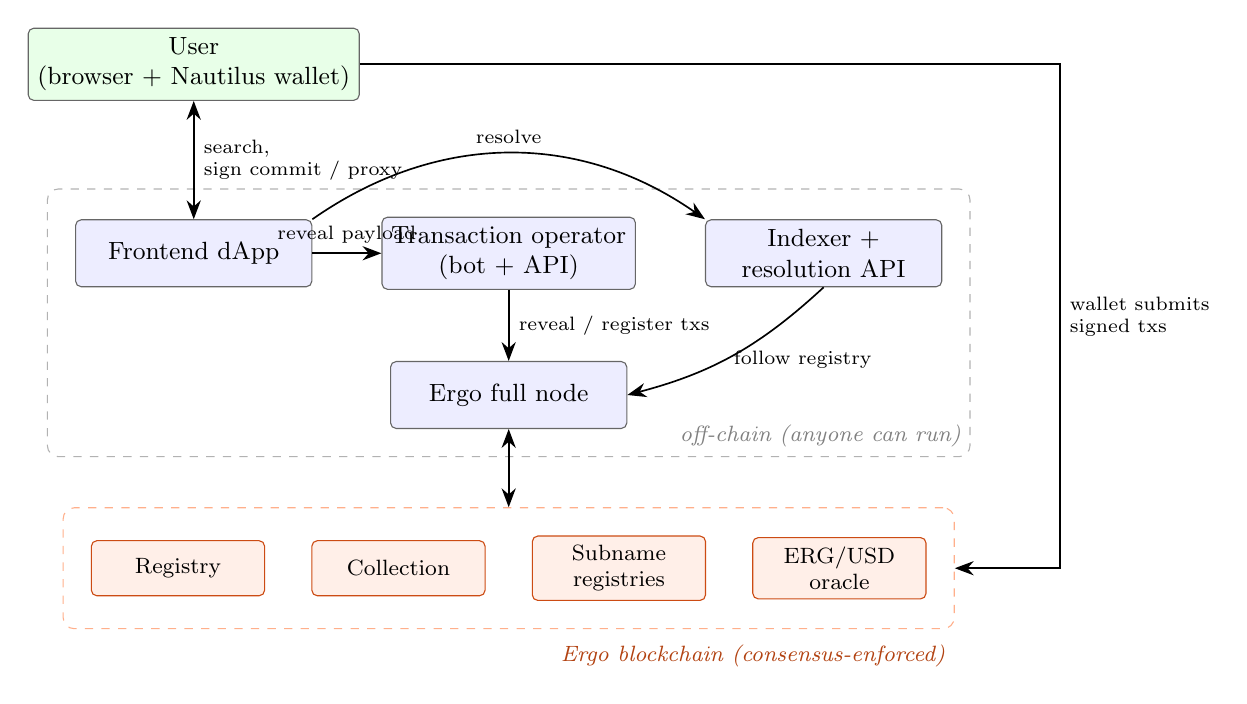
\begin{tikzpicture}[
  comp/.style={draw=black!60, fill=blue!7, rounded corners=2pt,
    minimum width=3.0cm, minimum height=0.85cm, align=center, font=\small},
  chainbox/.style={draw=ergoorange!80!black, fill=ergoorange!10, rounded corners=2pt,
    minimum width=2.2cm, minimum height=0.7cm, align=center, font=\footnotesize},
  zone/.style={draw=black!30, dashed, rounded corners=4pt, inner sep=10pt},
  zlbl/.style={font=\footnotesize\itshape, text=black!50},
  arr/.style={-{Stealth[length=2.4mm]}, semithick},
  barr/.style={{Stealth[length=2.4mm]}-{Stealth[length=2.4mm]}, semithick}
]
  % user layer
  \node[comp, fill=green!9] (user) at (-4.0,5.8) {User\\(browser + Nautilus wallet)};

  % off-chain services
  \node[comp] (frontend) at (-4.0,3.4) {Frontend dApp};
  \node[comp] (bot)      at (0,3.4)    {Transaction operator\\(bot + API)};
  \node[comp] (indexer)  at (4.0,3.4)  {Indexer +\\resolution API};
  \node[comp] (node)     at (0,1.6)    {Ergo full node};

  % on-chain layer
  \node[chainbox] (registry)   at (-4.2,-0.6) {Registry};
  \node[chainbox] (collection) at (-1.4,-0.6) {Collection};
  \node[chainbox] (subreg)     at (1.4,-0.6)  {Subname\\registries};
  \node[chainbox] (oracle)     at (4.2,-0.6)  {ERG/USD\\oracle};

  % zones
  \node[zone, fit=(frontend)(bot)(indexer)(node)] (offzone) {};
  \node[zlbl, anchor=south east] at (offzone.south east)
    {off-chain (anyone can run)};
  \node[zone, draw=ergoorange!50, fit=(registry)(collection)(subreg)(oracle)]
    (chainzone) {};
  \node[zlbl, anchor=north east] at ([yshift=-2pt]chainzone.south east)
    {\textcolor{ergoorange!70!black}{Ergo blockchain (consensus-enforced)}};

  % edges
  \draw[barr] (user.south) -- node[right, font=\scriptsize, align=left]
    {search,\\sign commit / proxy} (frontend.north);
  \draw[arr] (frontend.east) -- node[above, font=\scriptsize]
    {reveal payload} (bot.west);
  \draw[arr] (frontend.north east) to[bend left=35]
    node[above, font=\scriptsize, pos=0.5] {resolve} (indexer.north west);
  \draw[arr] (user.east) -- (7.0,5.8) --
    node[right, font=\scriptsize, align=left, pos=0.5]
    {wallet submits\\signed txs} (7.0,-0.6) -- (chainzone.east);
  \draw[arr] (bot.south) -- node[right, font=\scriptsize]
    {reveal / register txs} (node.north);
  \draw[arr] (indexer.south) to[bend left=14]
    node[right, font=\scriptsize, pos=0.55] {follow registry} (node.east);
  \draw[barr] (node.south) -- (node.south |- chainzone.north);
\end{tikzpicture}
\caption{Reference architecture. The chain enforces all protocol rules;
off-chain components provide only convenience and liveness, and any party can
run their own operator or indexer against the same on-chain registry.}
\label{fig:architecture}
\end{figure}

% ================= 10 =================
\section{Security Considerations}

\begin{itemize}
  \item \textbf{Front-running} is mitigated by commit--reveal with an
        enforced minimum commit age (\S\ref{sec:mintflow}).
  \item \textbf{Registry contention} is inherent to a singleton design: only
        one mint can advance the registry per transaction. The operator
        serializes registrations; throughput is bounded by block capacity,
        which is ample for a naming workload. Losers of any race are
        refunded.
  \item \textbf{Oracle dependence.} Pricing trusts the SigUSD oracle pool,
        Ergo's longest-running decentralized oracle. A bounded slippage
        window absorbs datapoint drift between quote and confirmation; the
        oracle is read-only (data input), so it cannot be manipulated within
        the mint transaction itself.
  \item \textbf{Operator compromise} cannot mint invalid names
        (consensus-validated), steal in-flight funds (user-signed refunds),
        or alter registrations (hash-bound reveals). The blast radius of a
        compromised operator key is limited to its own fee revenue and
        liveness.
  \item \textbf{Multisig compromise} could re-point protocol boxes to
        malicious logic for \emph{future} mints, but cannot touch existing
        names or in-flight user refund paths. Key-role separation (cold
        multisig distinct from the operator's hot key) is part of the launch
        hardening.
  \item \textbf{Name squatting} is an economic question rather than a
        protocol flaw under lifetime ownership; the length-tiered USD pricing
        makes mass-squatting short names expensive. The price map remains
        tunable as the market reveals itself.
  \item \textbf{Homoglyph/confusable attacks} are constrained by the
        deliberately minimal ASCII alphabet --- no Unicode, no mixed scripts,
        no punycode ambiguity.
\end{itemize}

% ================= 11 =================
\section{Comparison with Existing Naming Systems}

\begin{table}[ht]
  \centering
  \small
  \begin{tabularx}{\textwidth}{@{}>{\raggedright\arraybackslash}p{3.1cm} X X X@{}}
    \toprule
    & \textbf{ErgoNames} & \textbf{ENS (Ethereum)} & \textbf{DNS} \\
    \midrule
    Ownership model & Lifetime, one-time fee & Rental, annual renewal &
      Rental, annual renewal \\
    \addlinespace
    Expiry risk & None & Name lost if renewal lapses &
      Name lost if renewal lapses \\
    \addlinespace
    Uniqueness enforcement & Consensus (AVL proofs) & Contract storage &
      Registrar hierarchy \\
    \addlinespace
    Resolution & Token custody $=$ ownership $=$ resolution &
      Separate resolver records & Zone files \\
    \addlinespace
    Artwork/metadata & Fully on-chain SVG & Typically off-chain & n/a \\
    \addlinespace
    Subnames & Native, NFT per subname, parent-revocable &
      Supported via wrappers & Delegation \\
    \addlinespace
    Censorship of registration & Operator bypassable; rules
      consensus-enforced & Permissionless & Registrar policy \\
    \bottomrule
  \end{tabularx}
  \caption{ErgoNames compared with ENS and DNS.}
  \label{tab:comparison}
\end{table}

% ================= 12 =================
\section{Roadmap}

\begin{enumerate}
  \item \textbf{Launch (mainnet).} Fresh production genesis; public minting
        via the web dApp; resolution and reverse-resolution APIs;
        self-service refund tooling. The full mint, refund, pricing,
        fee-distribution, and upgrade machinery described in this paper is
        implemented and has been exercised end-to-end on Ergo mainnet.
  \item \textbf{Ecosystem integration.} Wallet-native resolution
        (send-to-\name{name}), reverse resolution as display identity,
        marketplace listing of the collection.
  \item \textbf{Subname tooling.} UI for minting, delegating, and revoking
        subnames.
  \item \textbf{Payment options.} Token-denominated payment via the config
        box and DEX price data inputs.
  \item \textbf{Progressive decentralization.} Expanded multisig key set and
        role separation; published runbooks enabling third-party operators
        and indexers.
\end{enumerate}

% ================= 13 =================
\section{Conclusion}

ErgoNames demonstrates that a complete naming protocol --- unique
registration, front-running resistance, oracle pricing, hierarchical
subnames, contract-enforced revenue splits, and safe upgradability --- can be
expressed in the eUTXO model with a footprint of one registry box and a
handful of small contracts. The design inverts the prevailing rental model: a
name is property, not a subscription. Ownership is token custody, resolution
is a consequence of ownership, and every artifact a name consists of lives
on-chain. The result is a naming layer with the permanence users expect from
the word \emph{name}.

\vspace{1cm}
\noindent\rule{\textwidth}{0.4pt}
\vspace{0.2cm}

\noindent\small
Contracts:
\href{https://github.com/ergonames/ergonames-contracts}{github.com/ergonames/ergonames-contracts}
(ErgoScript v1, source-available). Original contract author: Luca D'Angelo.
This document describes protocol version 1.

\end{document}
